\chapter{Methodology \& Results}

\section{Test Problem Generation} \label{Test_Problem}
The Solomon Benchmark \cite{solomon_algorithms_1987} contains problems random (R), clustered (C) and randomly clustered (RC). These describes how the customers are scattered around the terminal. These problems can be further broken down into type 1 and type 2 problems. Type 1 problems have a short scheduling horizon, allowing for only a few customers to be serviced by one vessel. In contrast, Type 2 problems have long scheduling horizon allowing many customers to be serviced by a vessel. Lastly, the problems are numbered from 1 upwards. Smaller numbered problems have customers with tight time windows, and larger numbered problems have time windows which are large. For example for problem R201, the first digit means that the customers are randomly scattered. The second digit represents that it is problem type 2 and the last 2 digits represent that the time windows are very tight for this problem.

Only type 2 problems are used for testing as the long scheduling horizon allows the barges to take multiple trips. To ensure problems are representative, only those with very tight or very loose time windows are used for testing.

However, the Solomon dataset is not able to fully replicate the bunker supply problem. It only has one demand type. To remedy this for each customer, fuel demand is randomly assigned to 1 of 5 possible fuel types. Also, service time is taken to be dependent on the total amount of fuel demanded by the vessel, instead of being a constant value for all vessels.

\section{Implementation}
Both the mathematical formulation and Adaptive Large Neighbourhood Search (ALNS) heuristic is implemented in the Python Programming Language. Both algorithms are run on a personal computer with CPU Intel i7-10510U.
Table \ref{tab:Problem_parameters} gives values for the problem parameters.\\

\begin{table}[h]
    \centering
    %\renewcommand{\arraystretch}{1.3} % Adjust row spacing
    \begin{tabular}{>{\raggedright}p{0.2\linewidth} p{0.4\linewidth} p{0.2\linewidth}}
        \toprule
        \textbf{Parameter} & \textbf{Description} &\textbf{Value}\\ 
        \midrule
        $\zeta$ & Cost per unit time to operate vessel & $0.1$\\ 
        
        $Price_{f}$ & Price of each fuel type $f$ & $[1,1,1,1,1]$\\ 
         
        $\beta$ & Rate of fuel transfer at depot compared against when at vessel & $0.2$ \\ 
                             
       	%M & Arbitrary large constant for MILP formulation& $1e8$\\ 
		
		$\mathcal{K}$ & Number of barges available & $3$\\
				
		$Q_{f}$ & Capacity of each compartment in barge carrying fuel type $f$ & $[50,50,50,50,50]$\\
        \bottomrule
    \end{tabular}
    \caption{Problem Parameters}
    \label{tab:Problem_parameters}
\end{table}

\subsection{MILP Implementation}
The mathematical formulation is implemented using a solver agnostic library Pyomo. A solver agnostic library is chosen as it would allow for testing of various different solvers to find the best one.
Gurobi version 12.0.0 is chosen as the solver as preliminary tests show it to perform the best, amongst a list of commercial and open source solvers, such as CPLEX, HiGHS and GLPK. This is within expectations as commercial solvers are known to be more performant than open source ones.
To ensure fairness when comparing against ALNS, the solver is limited to using only one thread of the CPU. To ensure reasonable computing times, the solver is set to a time limit of 1 hour or 3600s. All other solver settings are kept at the default.

\subsection{ALNS Implementation}
Due to the large number of parameters, it is difficult and time consuming to tune all the parameters. Thus, values for various parameters for ALNS are chosen according to previous literature \cite{yu_adaptive_2024}. Table \ref{tab:ALNS_parameters} provide a summary of all the parameters used for the ALNS algorithm. Due to randomness present in ALNS, results would differ slightly for repeated runs on the same problem. Thus, the average solution and time taken for 5 runs of the algorithm is reported.

\begin{table}[h]
    \centering
    %\renewcommand{\arraystretch}{1.3} % Adjust row spacing
    \begin{tabular}{lll} 
        \toprule
        \textbf{Parameter} & \textbf{Description} &\textbf{Value}\\ 
        \midrule
        $\mathcal{T}_{max}, \mathcal{T}_{min}$ & Starting and Ending Temperature for SA & $[50,10^{-3}]$\\ 
        
        $\alpha$ & Cooling rate for SA & $0.995$\\ 
         
        $l_{r}$ & Learning rate & $0.1$ \\ 
                             
       	$\mathcal{D}$ & Maximum Degree of Destruction & $0.3$\\ 
		
		$\sigma_1,\sigma_2,\sigma_3,\sigma_4 $ & Scores for updating operator weights 
				& $[1,0.5,0.25,0]$\\
		
		$\theta_{update}$ & Number of iterations to update operator weights & $0.005$	 \\
		
		$\theta_{nonImp}$ & Number of non-improving iterations & $0.2$\\
				
		$a,b$ & Shaw parameters & $[1,1]$\\
        \bottomrule
    \end{tabular}
    \caption{ALNS Parameters}
    \label{tab:ALNS_parameters}
\end{table}

\section{Experiment Design}
The quality of the solution would be based on a few metrics, mainly, objective function, solution time and Gap from best bounds (for MILP).

To ensure that the developed methods are effective, the methods would be put through 3 sets of experiments.
\begin{enumerate}
\item Methods are tested on a set of 6 different test cases, each test case hand crafted to test a particular constraint.
\item Methods are tested on the modified version of the Solomon Benchmark as described in Section \ref{Test_Problem}. The formulation is tested on small, medium and large instances with 25, 50 and 100 customers respectively.
\item ALNS is compared against best known solutions (BKS) from a similar problem. They are tested on small, medium and large instances with 25, 50 and 100 customers respectively.
\end{enumerate}

The $T_{B}$ column in MILP refers to the time taken to find the best solution, while $T$ is the time taken for the algorithm to terminate. $Gap_{o}$ refers to the gap in the solution between the ALNS and MILP methods. A negative $Gap_{o}$ would indicate that the solution found by ALNS is worse than MILP. $Gap_{o}$ is calculated such that it is comparable to Gap found by MILP. As such $Gap_{o}$ should always be lower than Gap, as it is impossible to be better than upper bound solution found by MILP.

\section{Experiment 1}
The objective of this experiment is to prove that both methods are able to provide good solutions for simple test cases. The 6 test cases are described in Table \ref{tab:Expt_1}. 

\begin{table}[h]
    \centering
    %\renewcommand{\arraystretch}{1.3} % Adjust row spacing
    \begin{tabular}{p{0.05\linewidth}>{\raggedright}p{0.25\linewidth} p{0.6\linewidth}}
        \toprule
        \textbf{Test Case}&\textbf{Name} & \textbf{Description} \\ 
        \midrule
    
	1& Travelling Salesman Problem (TSP) & To test if 1 barge can find the shortest route to visit 6 customers arranged in a circle around the terminal\\ \addlinespace
     
      2& Vehicle Routing Problem (VRP) & To test if 3 barges are able to find the optimal route to 18 customers\\\addlinespace
        
       3& Multi-Trip Vehicle Routing Problem (MTVRP) & To test if 1 barge is able to perform multiple trips to 18 customers \\ \addlinespace
        
        4& Multi-Commodity Vehicle Routing Problem (MCVRP)& To test if 3 barges are able to deliver to customers with different fuel types \\ \addlinespace
        
        5& Vehicle Routing Problem with Time Windows (VRPTW)& To test if 3 barges are able to deliver to customers with tight time windows, which define the route\\ \addlinespace
        
       6& Greedy Vehicle Routing Problem (GVRP)& To test if 1 barge is able to select the best customers to deliver to when it is not possible to service all customers\\ 
    \bottomrule
    \end{tabular}
    \caption{Experiment 1 Test Cases}
    \label{tab:Expt_1}
\end{table}

It is expected that both methods are able to quickly solve all 6 test cases, as they are set-up to be relatively simple. The results are given in Table \ref{tab:Results Expt_1} and the solutions found by ALNS of the test problems is in Figure \ref{Fig:Expt_1}.

\begin{table}[h]
    \centering
    %\renewcommand{\arraystretch}{1.3} % Adjust row spacing
    %\setlength\tabcolsep{3pt}
    \begin{tabular}
    {c|S[table-format=3.2]S[table-format=2.2]S[table-format=1.2]S[table-format=3.2]|S[table-format=3.2]S[table-format=1.2]S[table-format=2.2]}
    %{p{0.08\linewidth} p{0.05\linewidth} | p{0.08\linewidth}p{0.05\linewidth}p{0.08\linewidth}p{0.08\linewidth}| p{0.08\linewidth}p{0.05\linewidth} p{0.08\linewidth}p{0.08\linewidth}}
        \toprule
        {\textbf{Test}} & \multicolumn{4}{c|}{\textbf{MILP}} & \multicolumn{3}{c}{\textbf{ALNS}}\\ 
     \textbf{Case} &  {Solution} & {$T_{B}$(s)} & {Gap(\%)} & {$T$(s)} &  {Solution} & {$T$(s)} & {$Gap_{o}$(\%)} \\
        \hline
    1 &  56.94 & 0.02 & 0.00 & 0.02 &  56.94 & 0.61 & 0.00  \\
    2 & 163.12 & 1    & 0.00 &61.79 & 163.12 & 1.95 & 0.00 \\
    3 & 163.12 & 2    & 2.80 & 180  & 163.12 & 1.72 & 0.00  \\
    4 & 155.70 & 15   & 5.04 & 180  & 155.80 & 2.85 & 0.06 \\
    5 & 104.59 & 56   &61.15 & 180  & 104.59 & 2.35 & 0.00 \\
    6 &  37.52 & 0.04 & 0.00 & 0.04&  37.52  & 0.71 & 0.00  \\
    
    \bottomrule
    \end{tabular}
    \caption{Results for Experiment 1}
    \label{tab:Results Expt_1}
\end{table} 

It can be seen that both MILP and ALNS methods are able to given similar results for the test cases. MILP is able to prove optimality solution for 3 out of the 6 test cases. The results prove that both methods are able to handle the constraints in the bunker supply problem appropriately.

\begin{figure} 
\begin{subfigure}{.5\textwidth}
	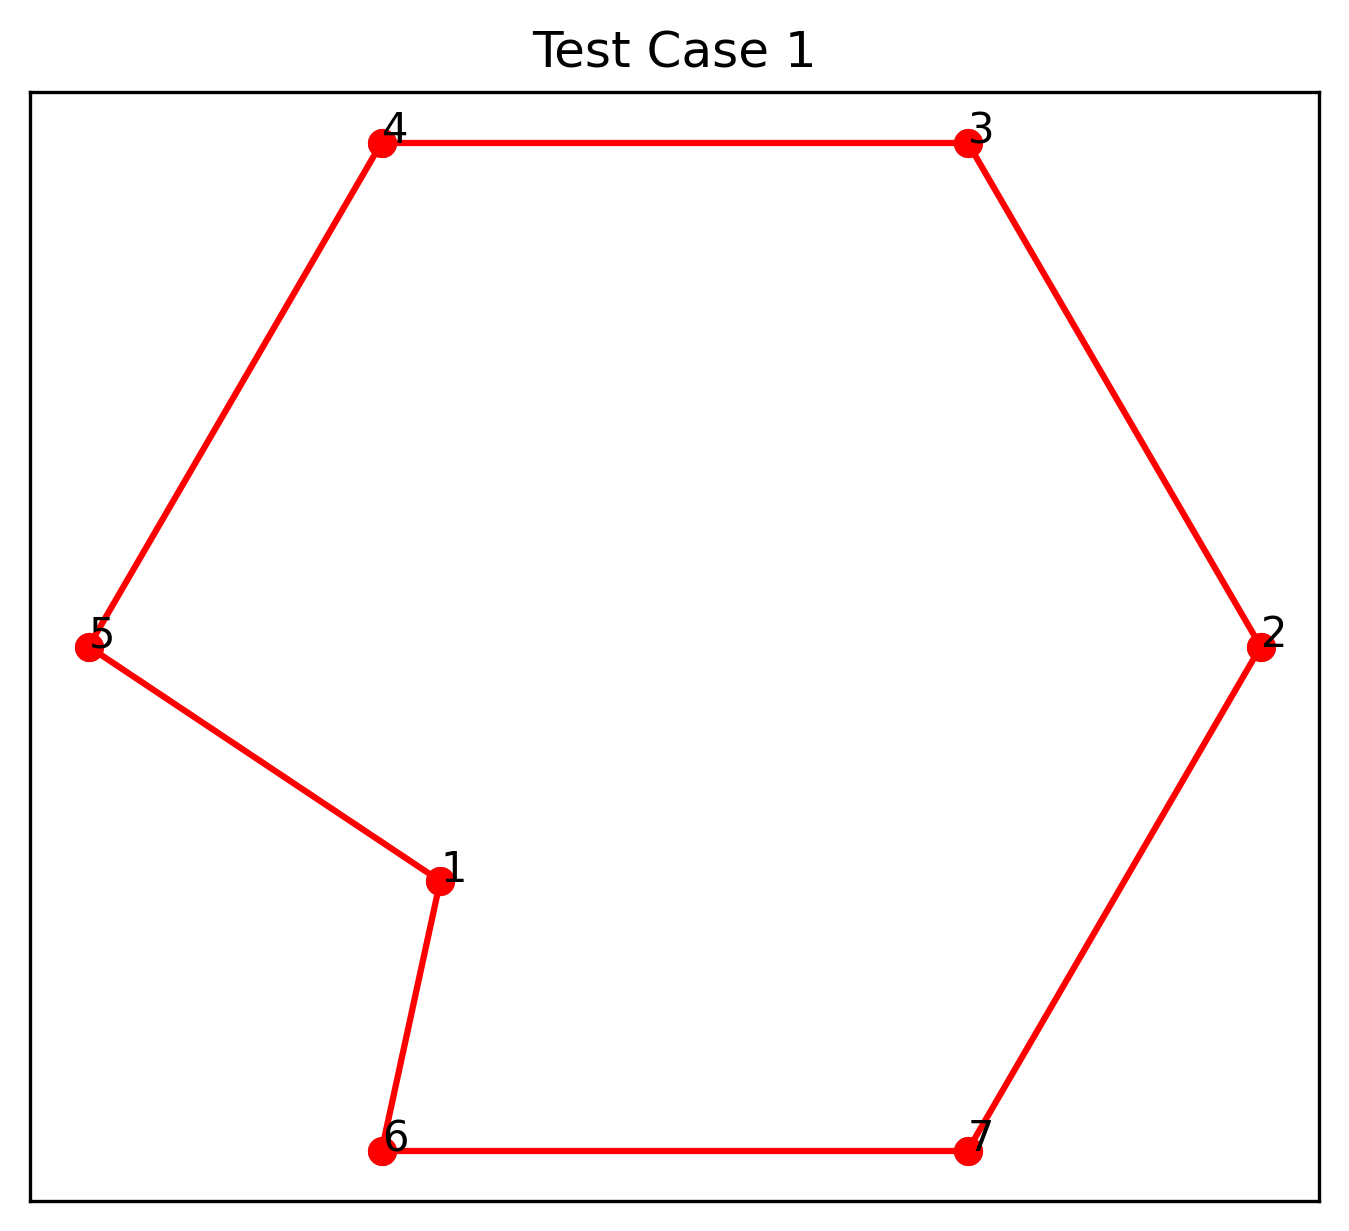
\includegraphics[scale=0.6]{TC_1.png}
\end{subfigure}
\begin{subfigure}{.5\textwidth}
	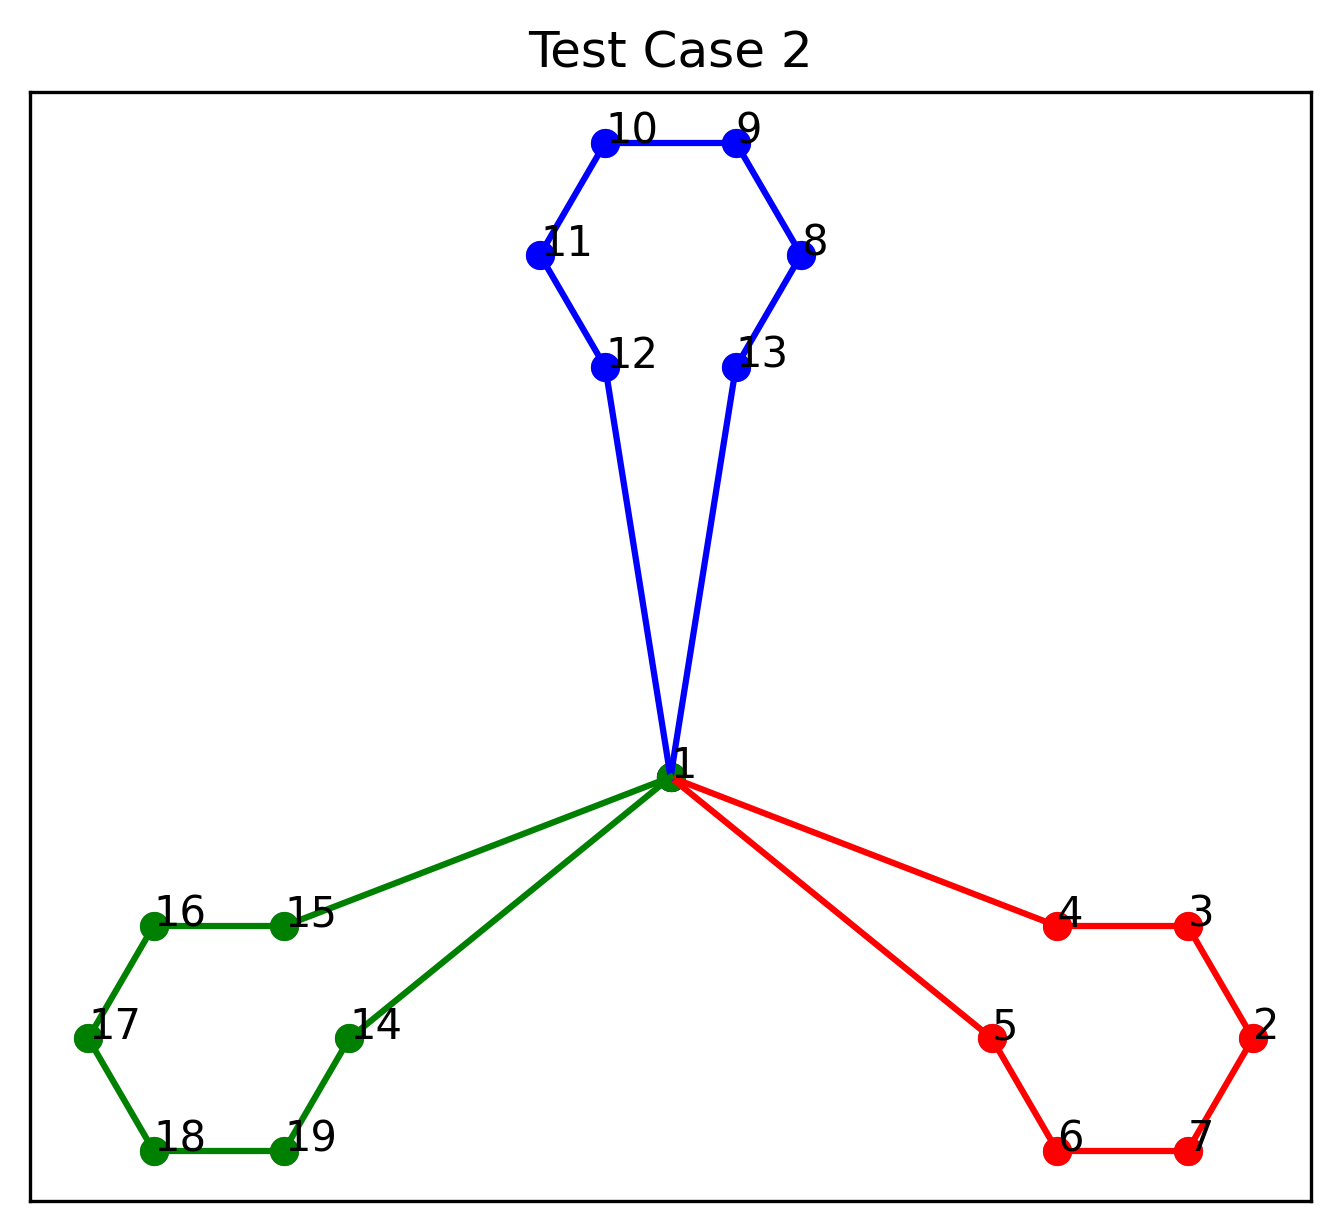
\includegraphics[scale=0.6]{TC_2.png}
\end{subfigure}

\begin{subfigure}{.5\textwidth}
	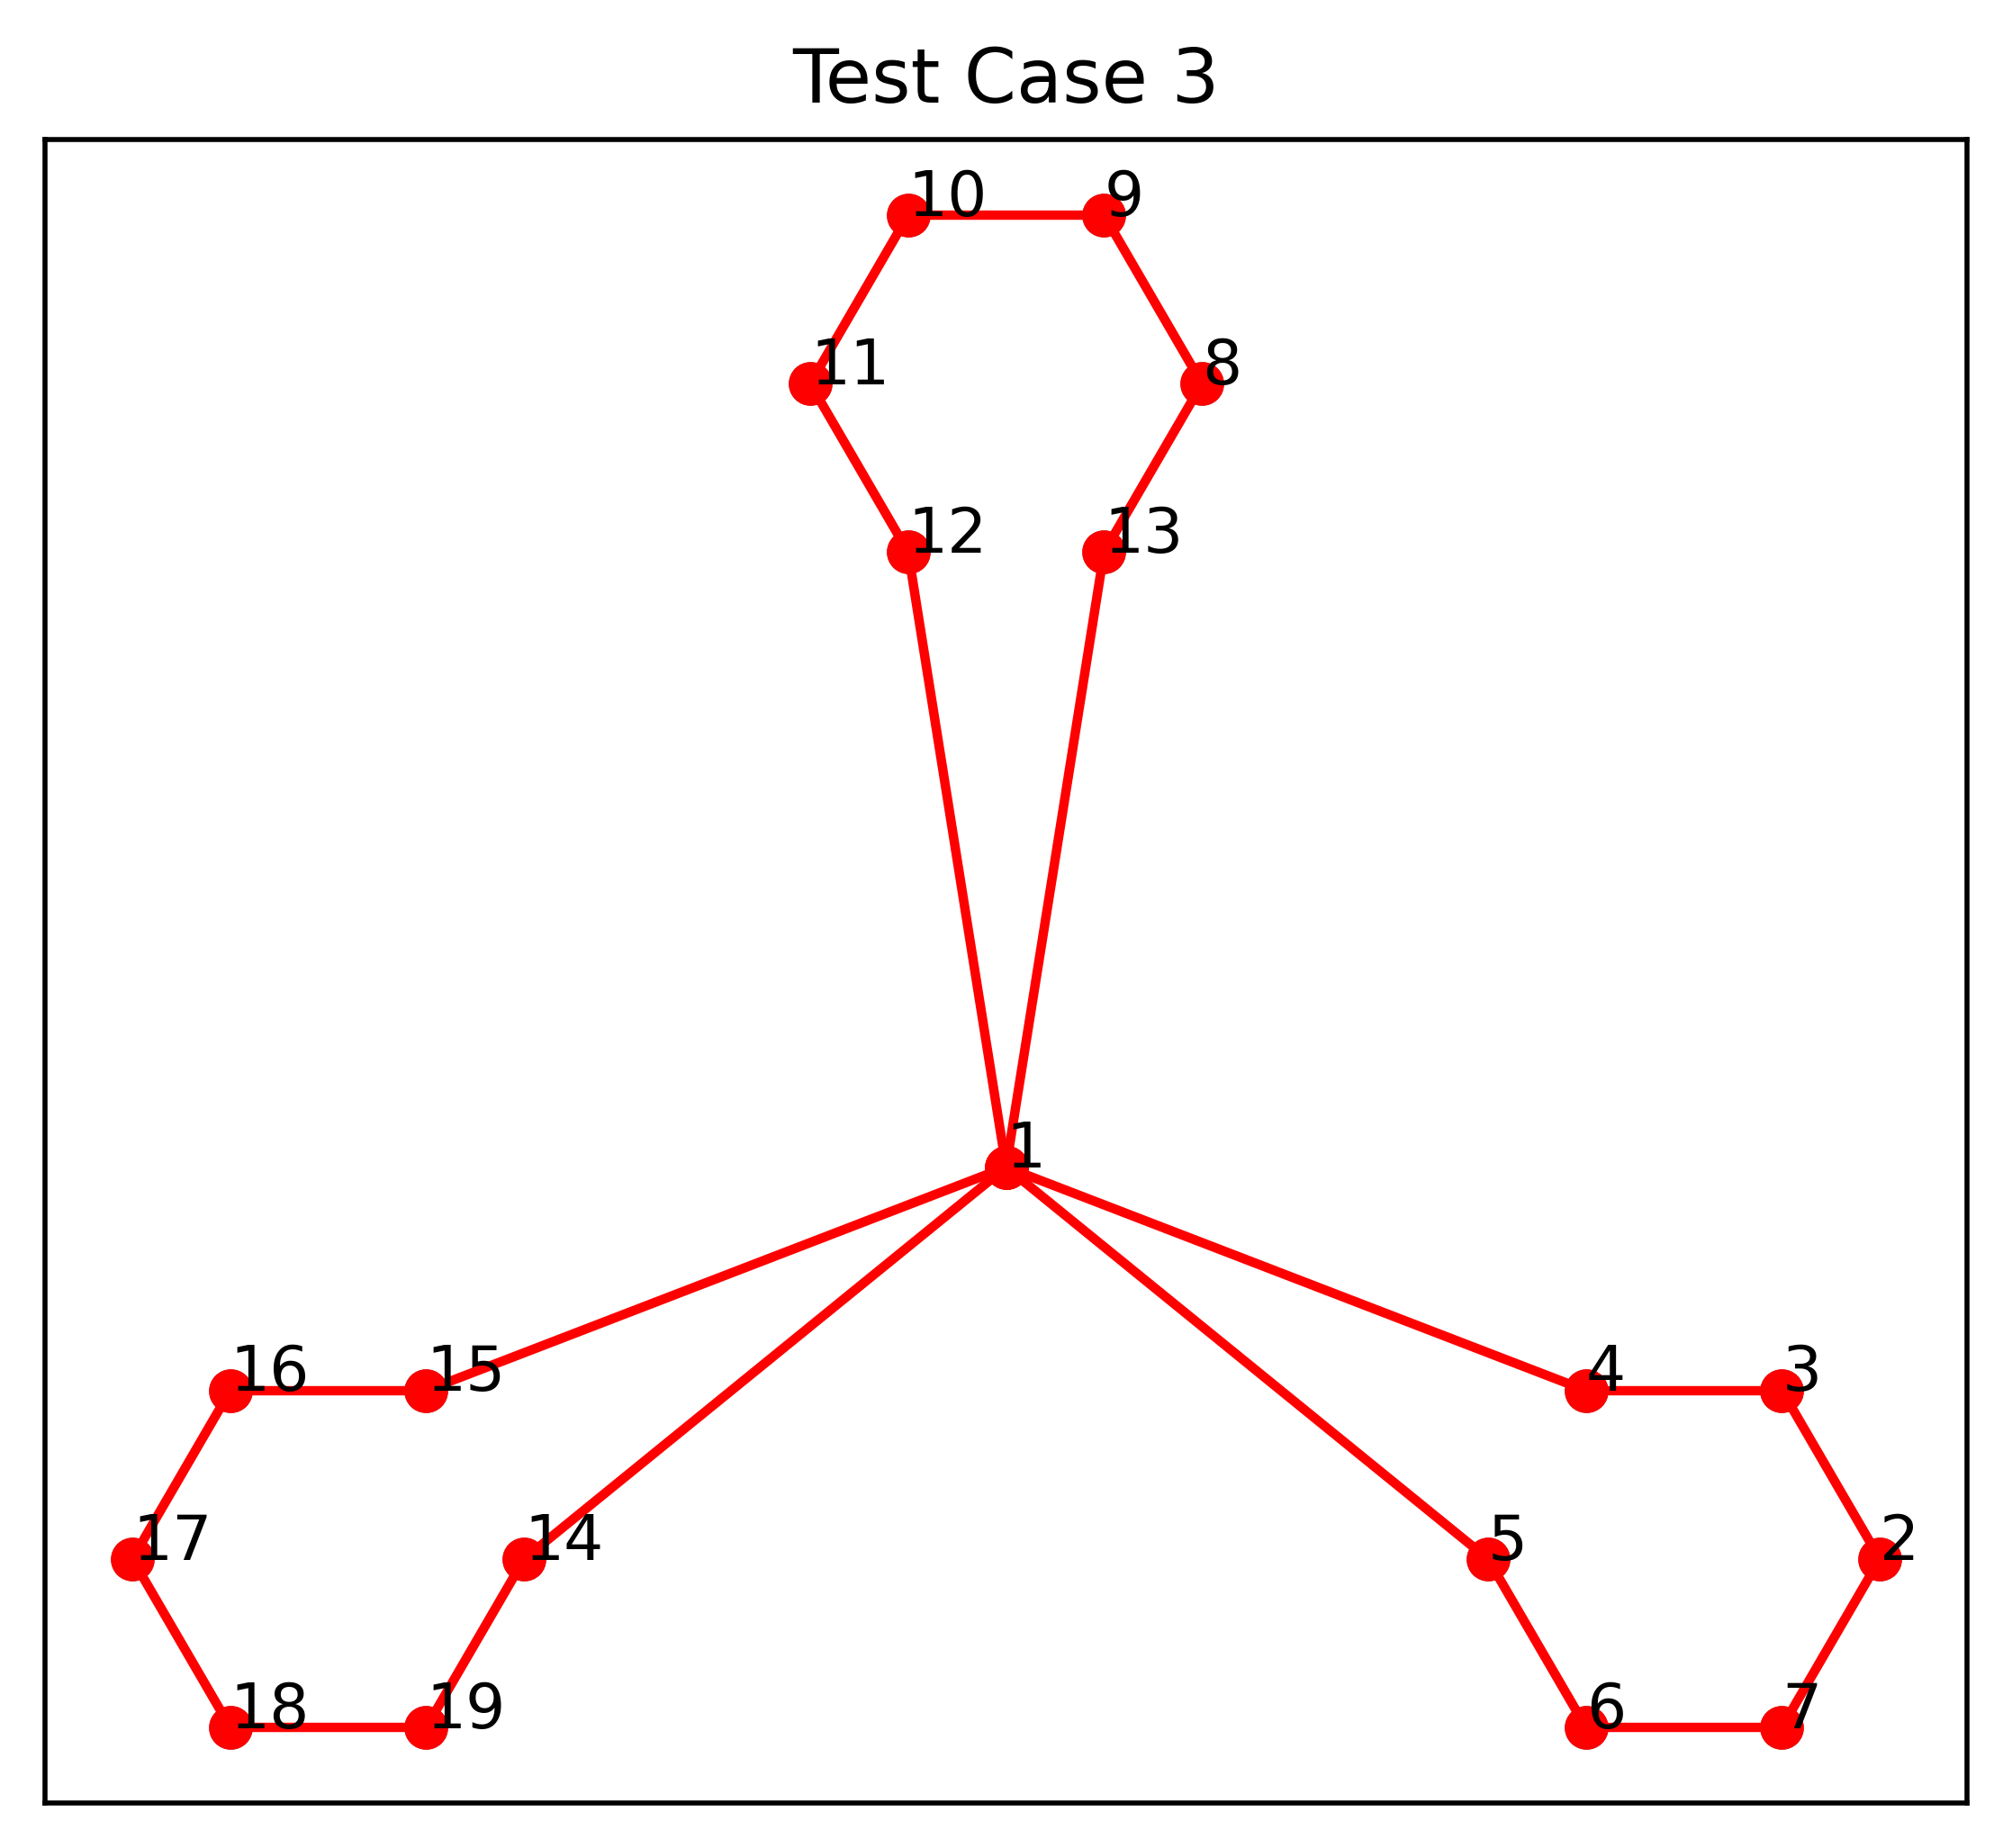
\includegraphics[scale=0.6]{TC_3.png}
\end{subfigure}
\begin{subfigure}{.5\textwidth}
	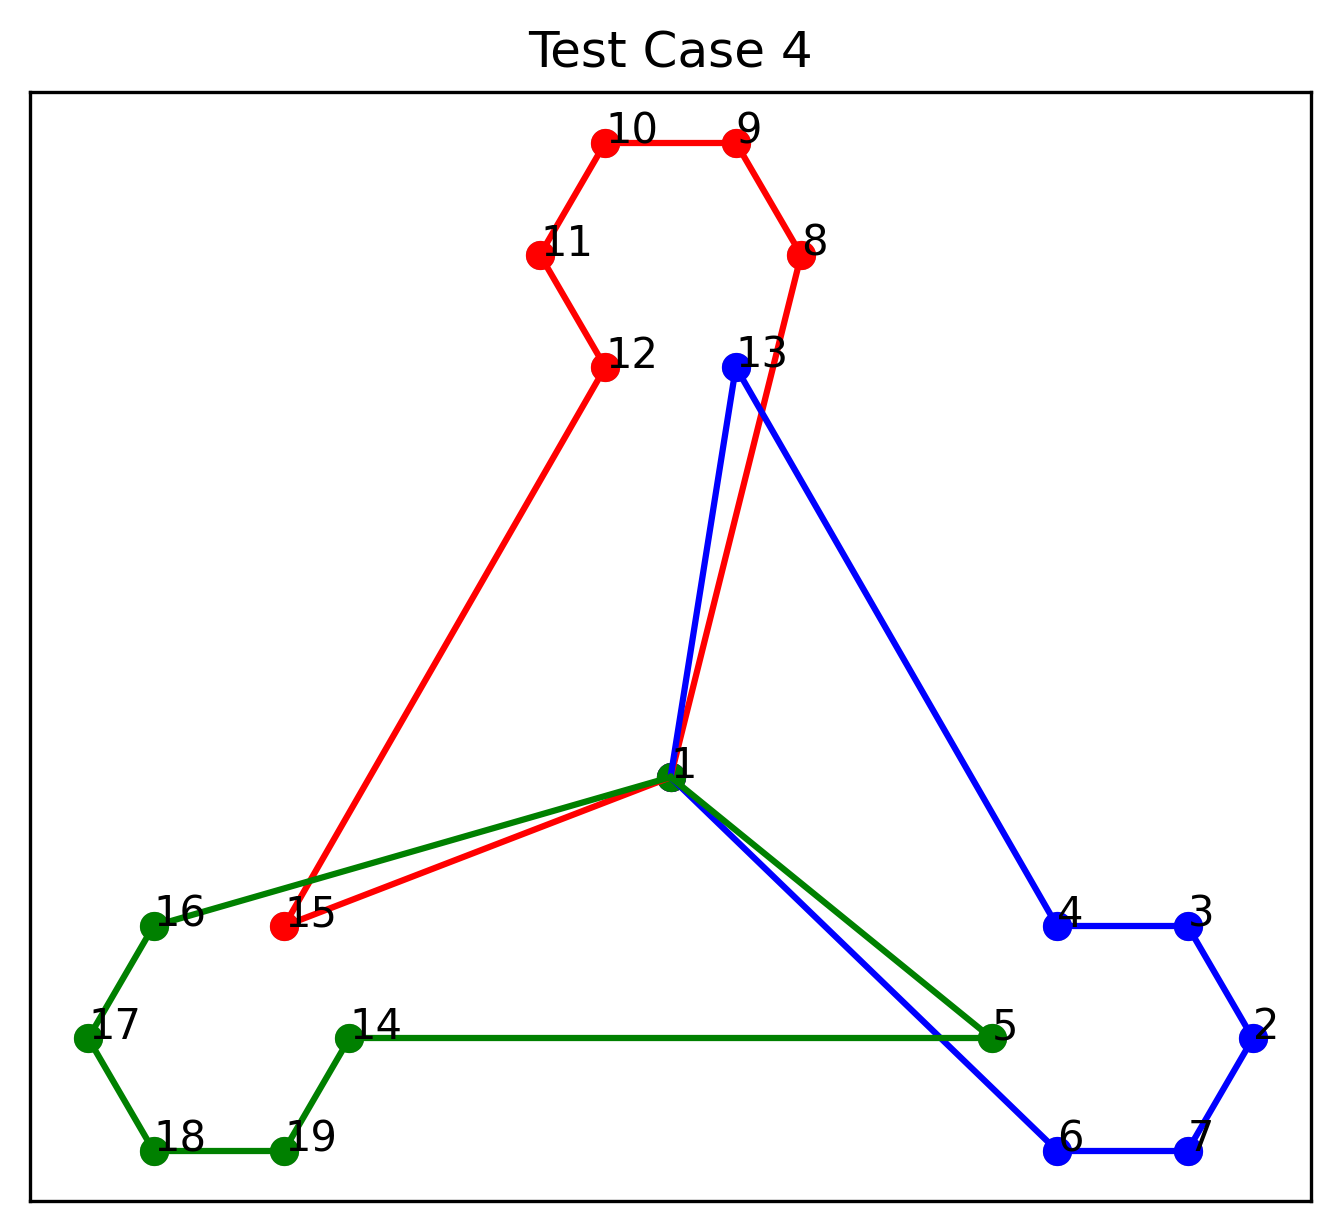
\includegraphics[scale=0.6]{TC_4.png}
\end{subfigure}

\begin{subfigure}{.5\textwidth}
	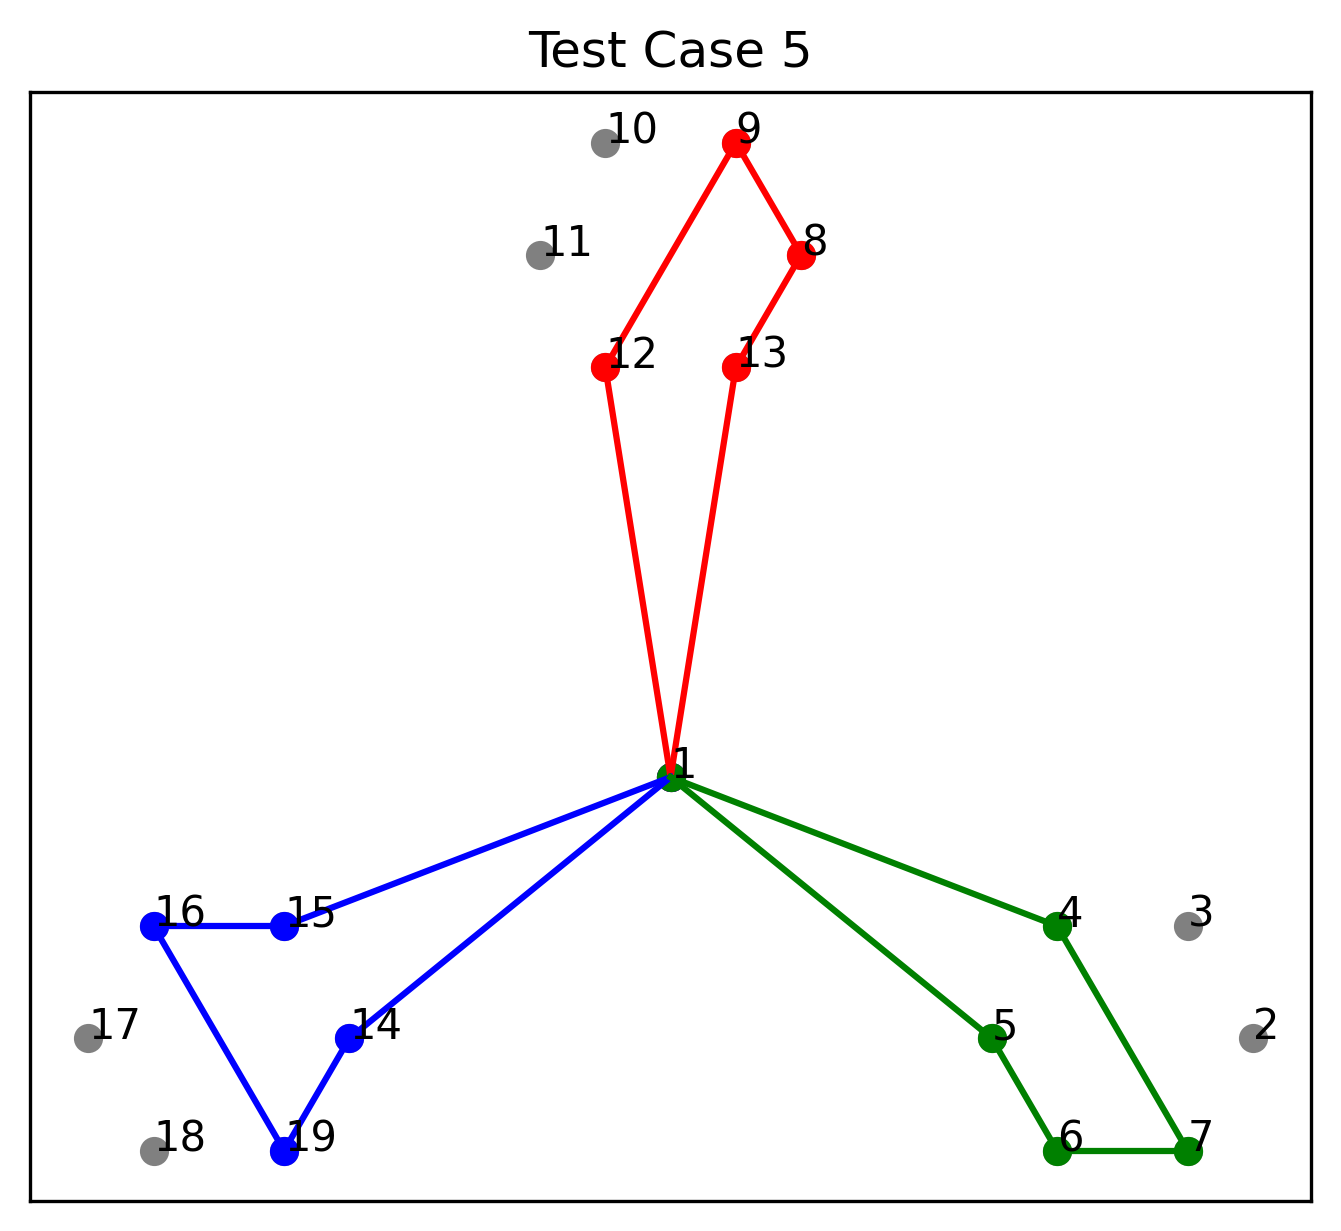
\includegraphics[scale=0.6]{TC_5.png}
\end{subfigure}
\begin{subfigure}{.5\textwidth}
	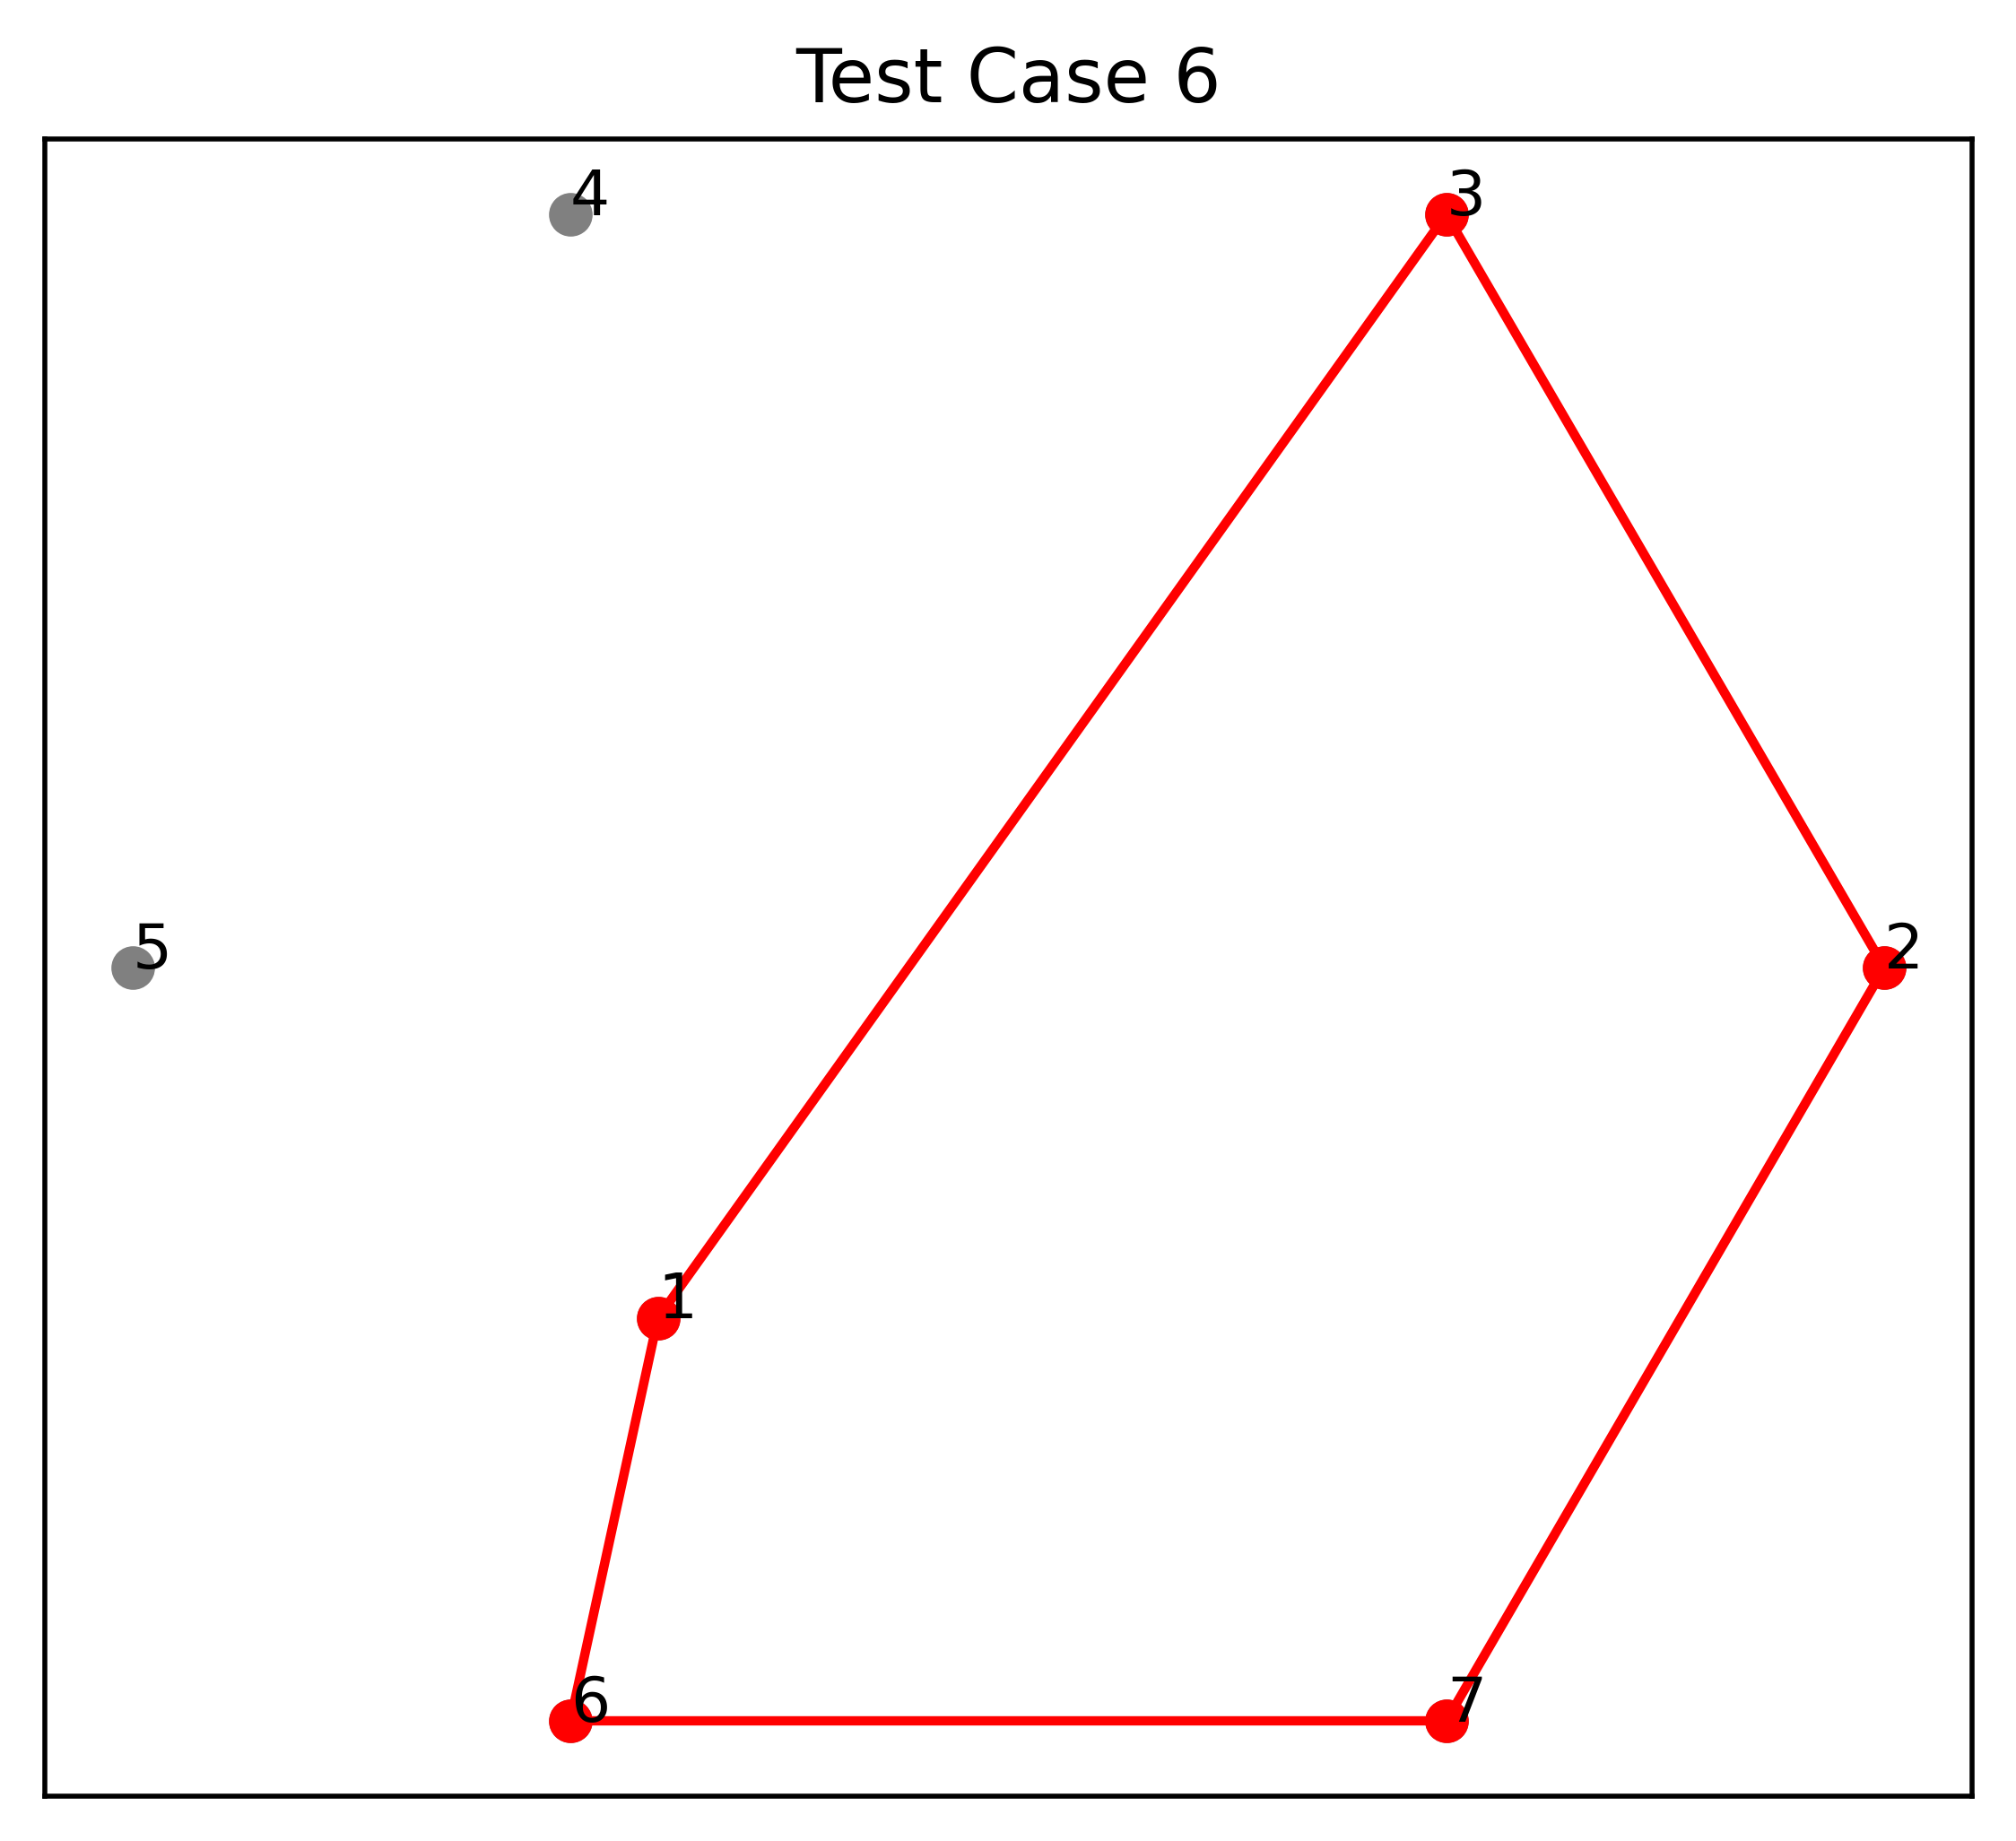
\includegraphics[scale=0.6]{TC_6.png}
\end{subfigure}
\caption{Experiment 1 routes obtained from ALNS} \label{Fig:Expt_1}
\end{figure} 

\section{Experiment 2}
The objective of this experiment is to test the relative performance between the 2 methods. This would allow us to compare the 2 methods and determine the strengths and weakness between the 2 approaches. The results are given in table \ref{tab:Results Expt_2} and a sample of the results obtained using ALNS for small test cases are shown in Figure \ref{Fig:Expt_2}.

\begin{table}[h]
    \centering
    %\renewcommand{\arraystretch}{1.3} % Adjust row spacing
    %\setlength\tabcolsep{3pt}
    \begin{tabular}
    {cc|S[table-format=3.2]rS[table-format=1.2]S[table-format=3.1]| S[table-format=3.2]S[table-format=2.2]S[table-format=2.2]}
    %{p{0.08\linewidth} p{0.05\linewidth} | p{0.08\linewidth}p{0.05\linewidth}p{0.08\linewidth}p{0.08\linewidth}| p{0.08\linewidth}p{0.05\linewidth} p{0.08\linewidth}p{0.08\linewidth}}
        \toprule
        {\textbf{Test}} &\multirow{2}{*}{\textbf{N}}& \multicolumn{4}{c|}{\textbf{MILP}} & \multicolumn{3}{c}{\textbf{ALNS}}\\ 
     \textbf{Case} & &  {Solution} & {$T_{B}$(s)} & {Gap(\%)} & {$T$(s)} & {Solution} & {$T$(s)} & {$Gap_{o}$(\%)} \\% & $Gap_{t}$(\%) \\
        \hline
    C201 & 25 & 432.81 & 3    & 0.00 & 77.66& 432.81 & 3.26 & 0.00 \\% & 180.31\\
    C208 & 25 & 432.88 & 377  & 1.43 & 3600 & 432.88 & 4.13 & 0.00 \\%& -97.47\\
    R201 & 25 & 284.34 & 2    & 0.00 &163.04& 282.97 & 4.13 & -0.48 \\%& 284.12\\
    R211 & 25 & 295.46 & 2259 & 1.71 & 3600 & 294.61 & 3.78 & -0.29 \\%& -99.64\\
    RC201 & 25& 490.51 & 87   & 0.00 &555.46& 487.10 & 5.07 & -0.70 \\%& -87.55 \\
    RC208 & 25& 494.95 & 1640 & 6.65 & 3600 & 496.55 & 4.21 & 0.32 \\%& -99.34 \\
    
    \hline
	C201 & 50 & 795.13 & 3430 & 2.76 & 3600 & 796.62 & 13.31 & 0.19 \\%& -98.52\\
    C208 & 50 & 796.05 & 3349 & 3.60 & 3600 & 803.97 & 15.01 & 1.00 \\%& -97.65\\
    R201 & 50 & 615.14 & 3069 & 4.05 & 3600 & 627.58 & 12.69 & 2.02 \\%& -98.57\\
    R211 & 50 & 647.15 & 3420 & 4.38 & 3600 & 657.48 & 12.21 & 1.60 \\%& -98.38\\
    RC201 & 50& 734.09 & 2774 &21.21 & 3600 & 794.32 & 18.65 & 8.21 \\%& -97.65\\
    RC208 & 50& 799.39 & 2978 &18.65 & 3600 & 884.22 & 14.31 &10.61 \\%& -97.77\\
    
    \hline
	C201 & 100& 1360.83& 3561 &28.22 & 3600 &1593.14 &  85.25 &17.07 \\%& -84.39\\
    C208 & 100& 1253.37& 3560 &39.99 & 3600 &1681.41 &  68.87 &34.15 \\%& -84.02\\
    R201 & 100& 830.81 & 3140 &61.76 & 3600 &1040.57 &  87.83 &25.25 \\%& -85.33\\
    R211 & 100& 776.26 & 3130 &79.78 & 3600 &1328.46 &  77.23 &71.14 \\%& -82.26\\
    RC201 &100& 853.46 & 3378 &86.77 & 3600 &1035.33 &  87.96 &21.31 \\%& -87.96\\
    RC208 &100& 801.67 & 3556 &107.58& 3600 &1338.63 &  94.36 &66.98 \\%& -83.26\\
        
    \bottomrule
    \end{tabular}
    \caption{Results for Experiment 2}
    \label{tab:Results Expt_2}
\end{table} 

\begin{figure} 
\begin{subfigure}{.5\textwidth}
	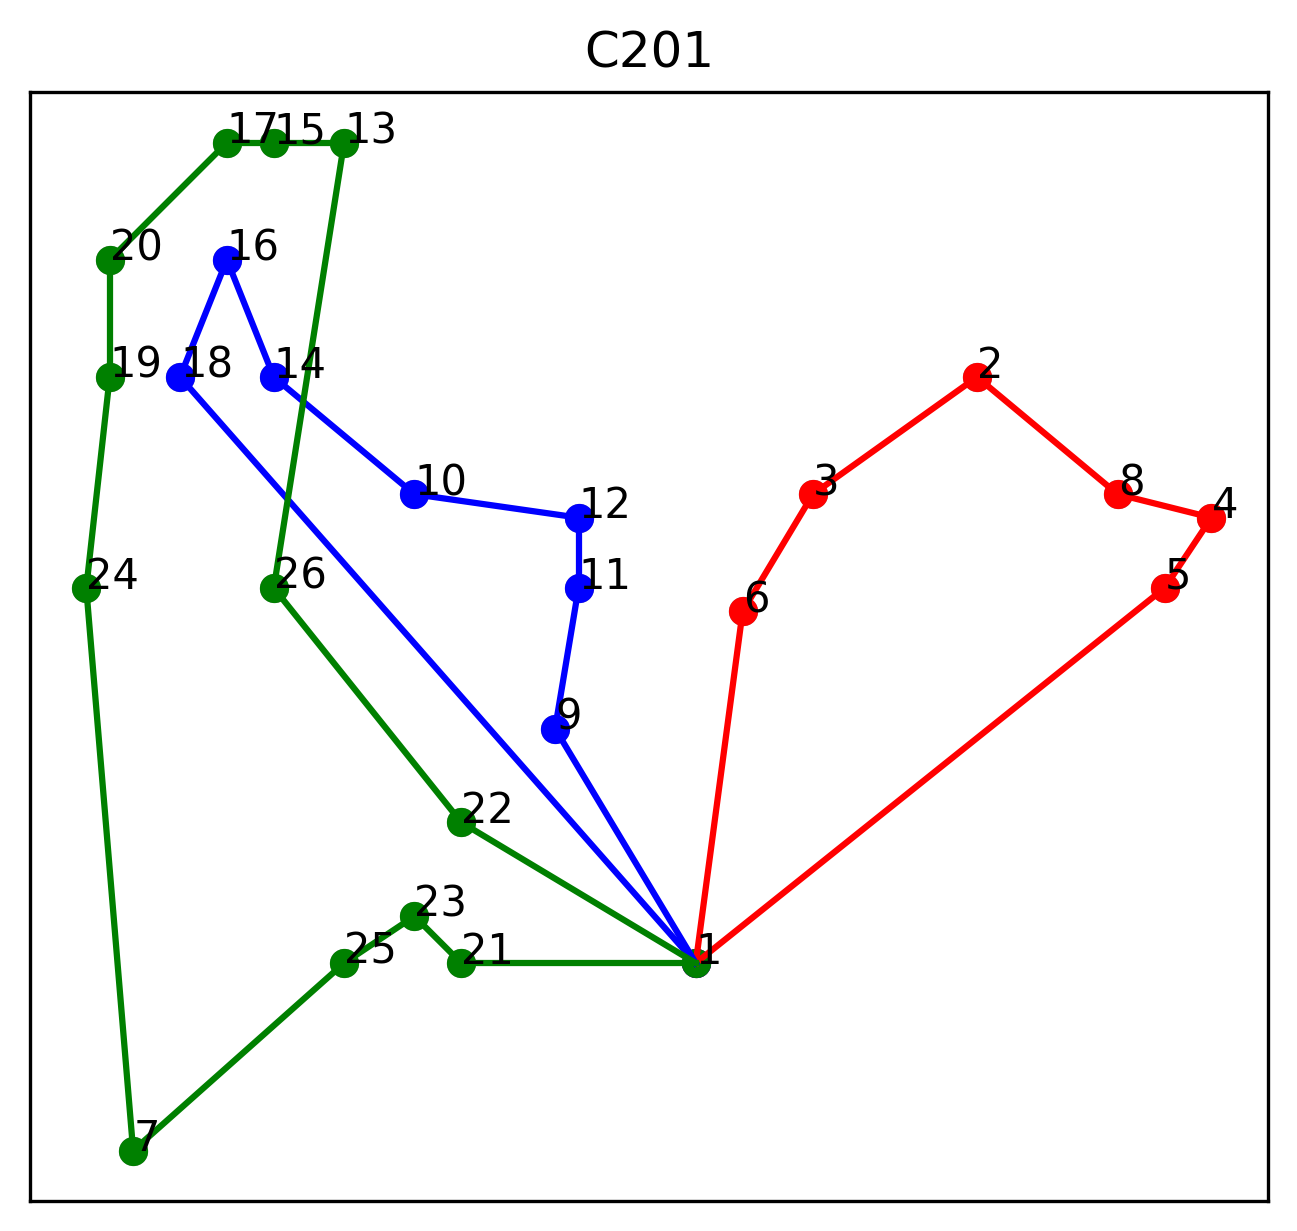
\includegraphics[scale=0.6]{C201.png}
\end{subfigure}
\begin{subfigure}{.5\textwidth}
	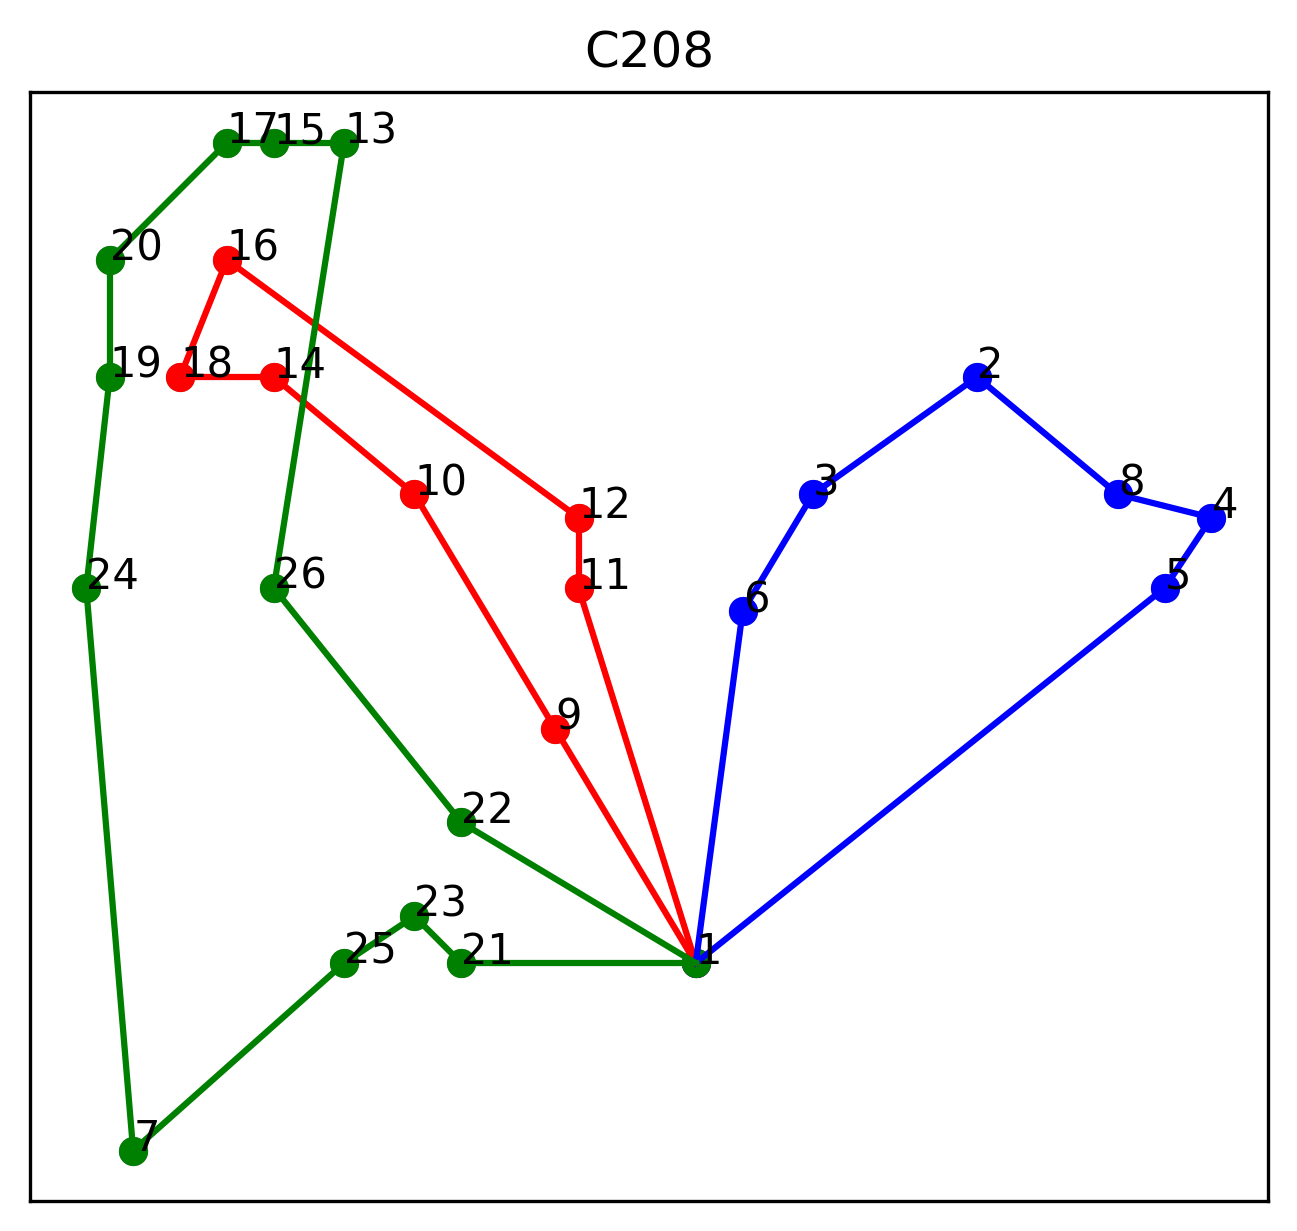
\includegraphics[scale=0.6]{C208.png}
\end{subfigure}

\begin{subfigure}{.5\textwidth}
	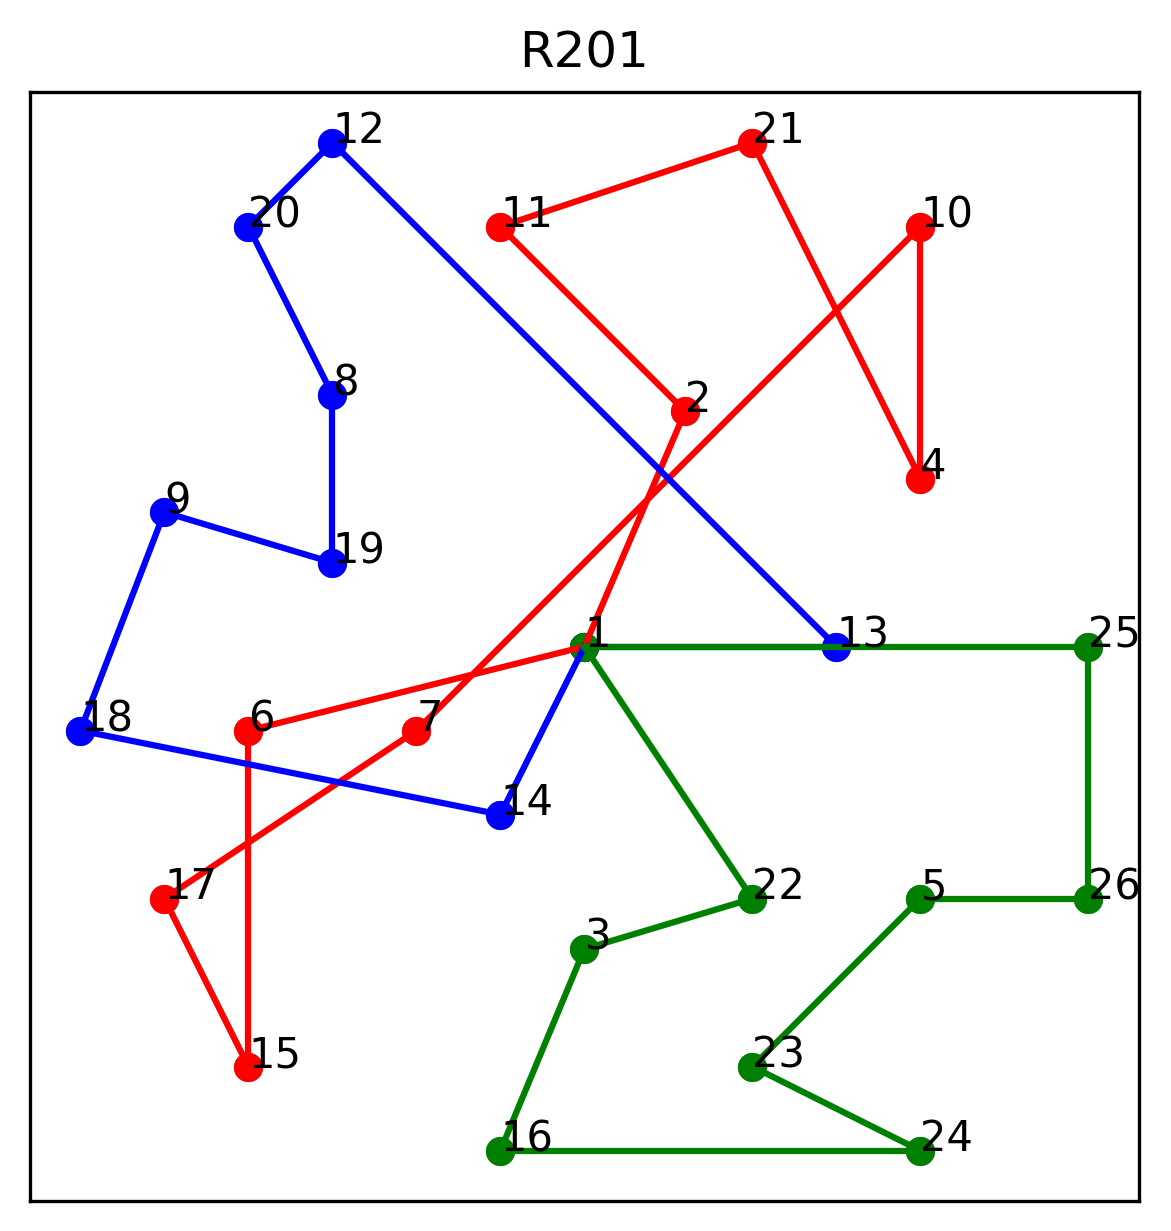
\includegraphics[scale=0.65]{R201.png}
\end{subfigure}
\begin{subfigure}{.5\textwidth}
	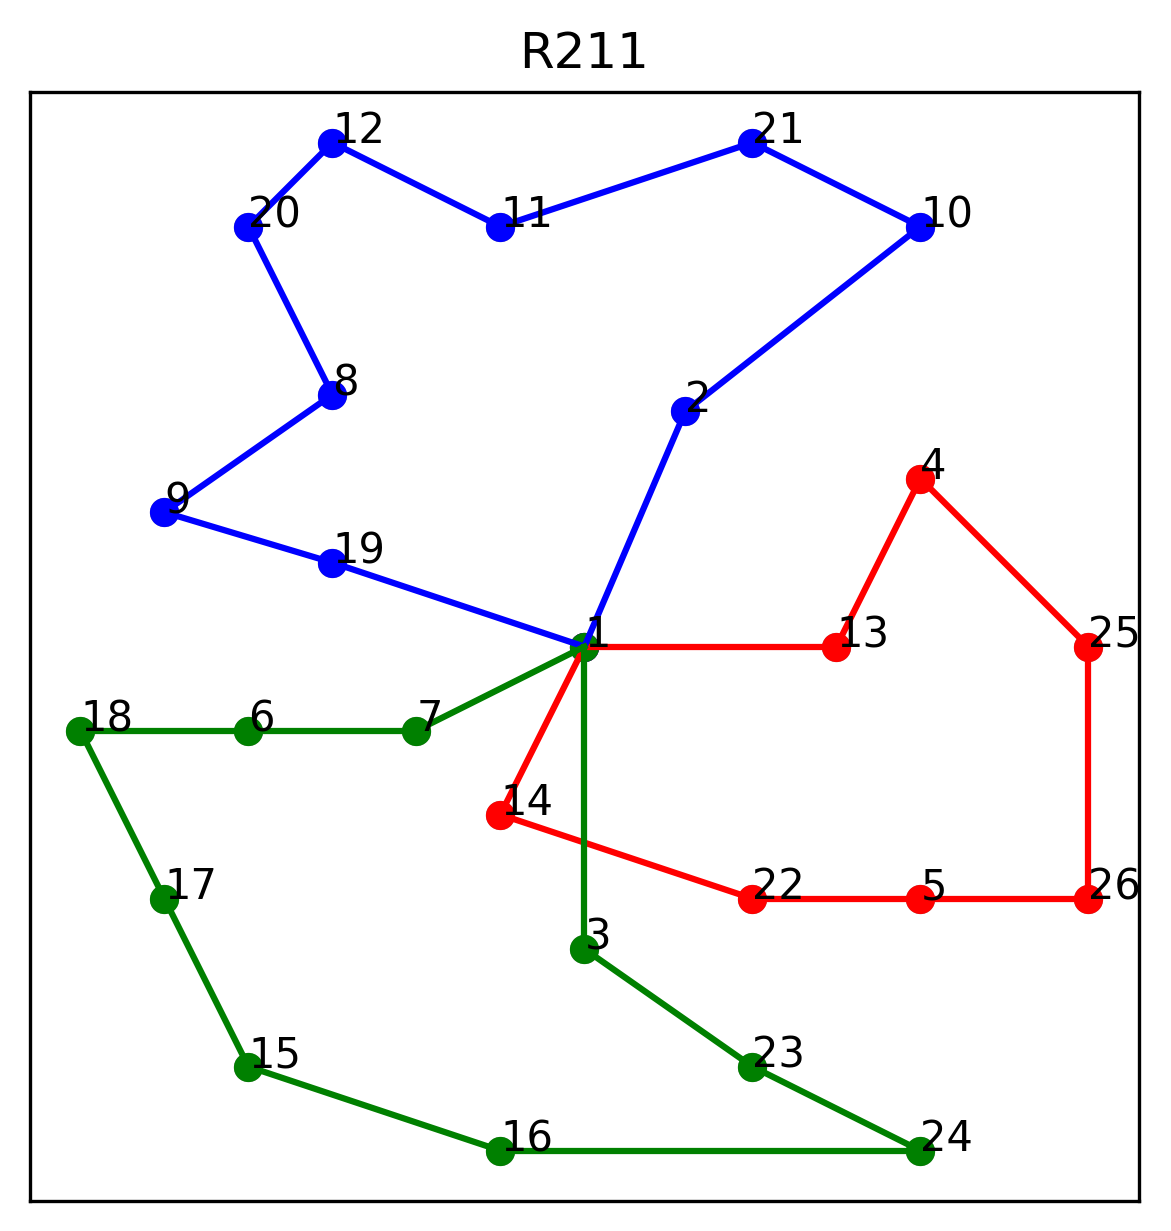
\includegraphics[scale=0.65]{R211.png}
\end{subfigure}

\begin{subfigure}{.5\textwidth}
	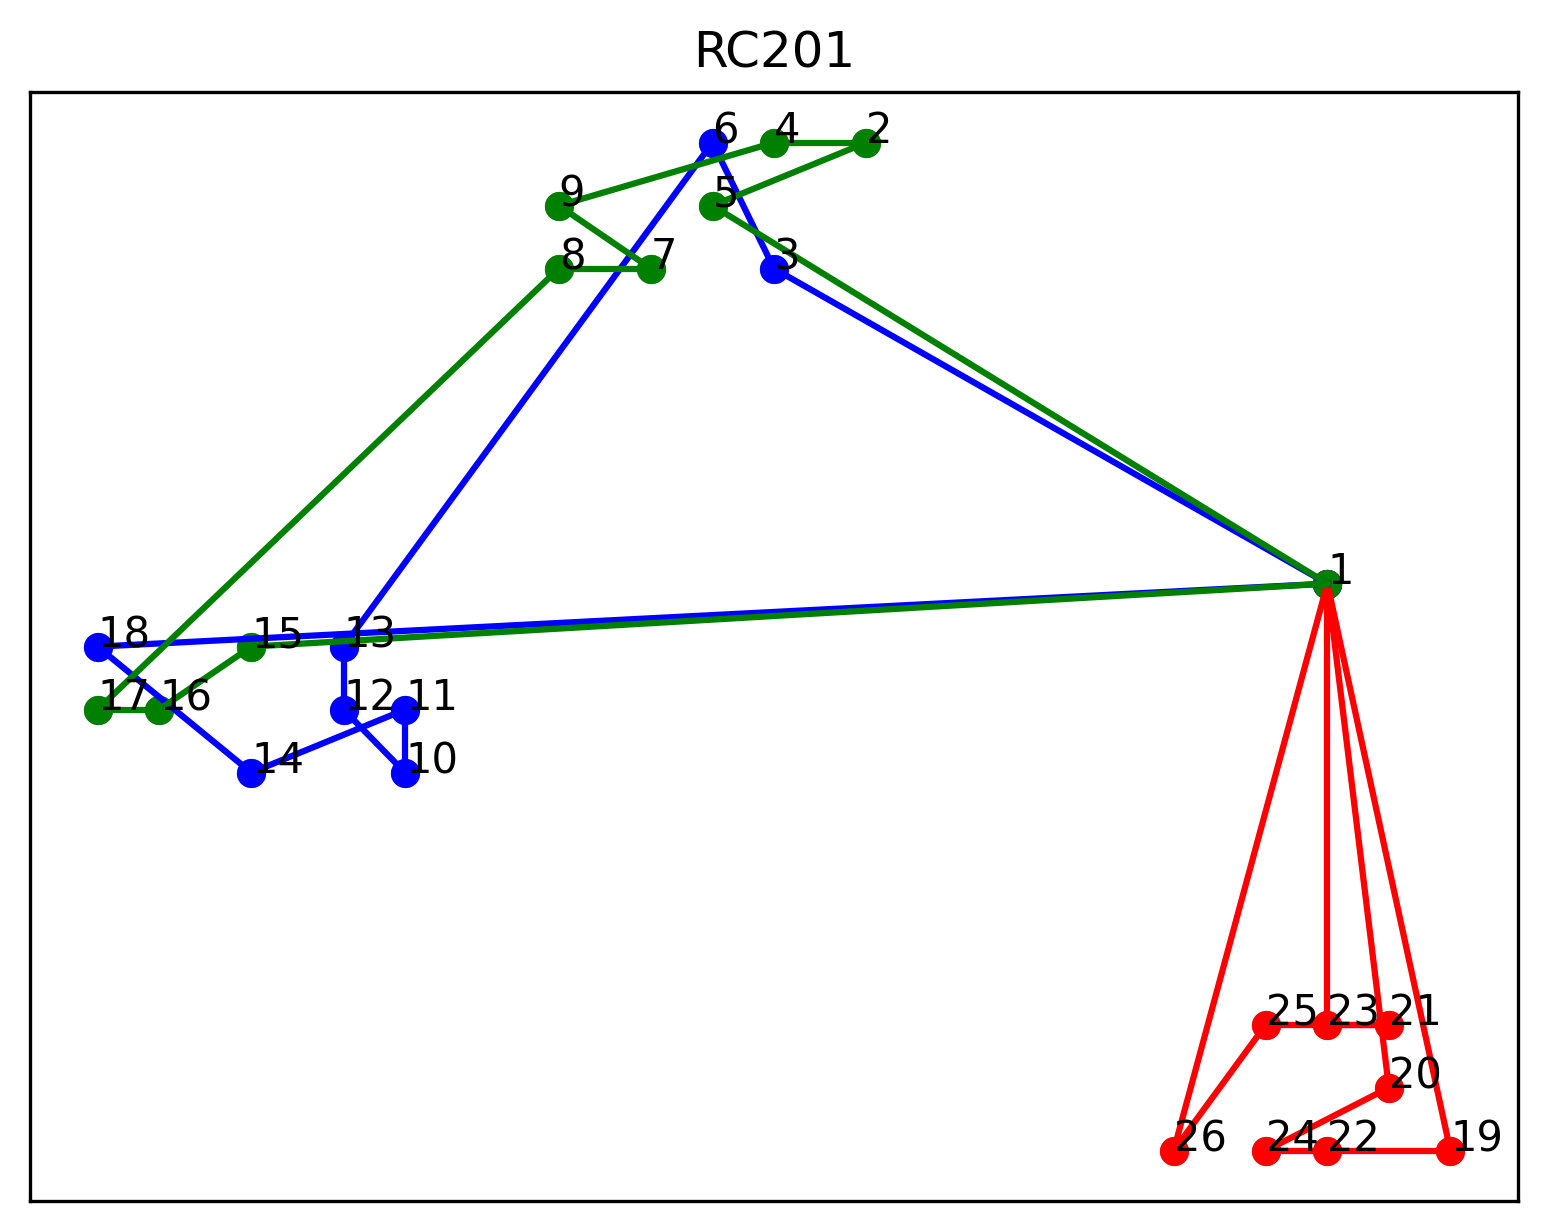
\includegraphics[scale=0.5]{RC201.png}
\end{subfigure}
\begin{subfigure}{.5\textwidth}
	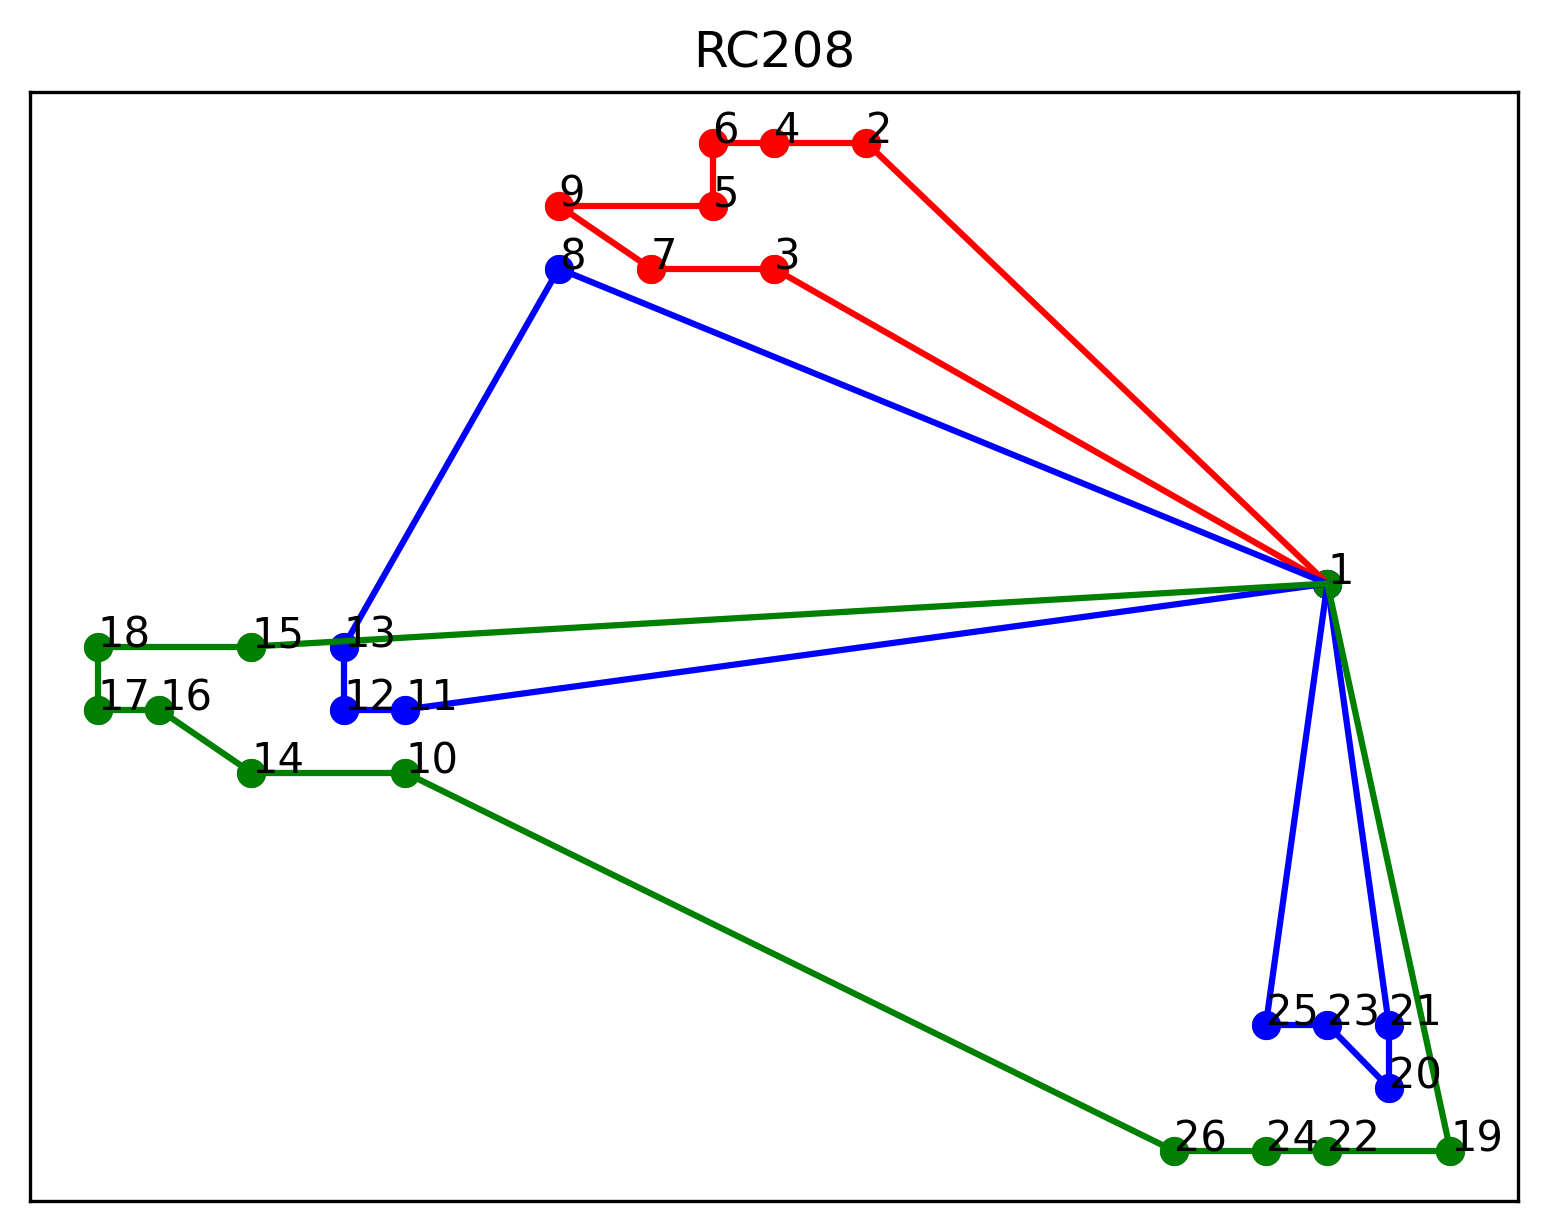
\includegraphics[scale=0.5]{RC208.png}
\end{subfigure}
\caption{Experiment 2 routes obtained from ALNS for small test cases} \label{Fig:Expt_2}
\end{figure} 

For small test instances ($N=25$) both methods are able to find optimal or close to the optimal solution however, solution time is much more stable for ALNS, varying between 3.26 and 5.07 seconds. In contrast MILP takes betwen 77.66 and 3600 seconds to terminate.

For medium test instances ($N=50$) ALNS in general slightly outperforms MILP method, being able to find slightly better solutions for all test cases in  much quicker time. However, MILP is able to show that the solutions found are still relatively close to optimal for at least 4 of the 6 test cases.

For large test instances ($N=100$) ALNS has a clear advantage over MILP in terms of both solution quality and solution time. However, due to the large upper bound gap produced by MILP, it is difficult to ascertain if the solutions produced by ALNS is close to the optimal solution.

These results show that ALNS is the superior method with its advantage increasing as the test problem size increases. 


\section{Experiment 3}
The objective of this experiment is to test the performance of ALNS against the best known solutions (BKS) \cite{yang_exact_2023} to evaluate its effectiveness. Given the results from Experiment 2, the ALNS method is proven to be superior and is thus used as a point of comparison against Best Known Solutions (BKS). Specifically, published results from the Capacitated Multi-Trip Vehicle Routing Problem with Time Windows - Loading Times (CMTVRPTW-LT) problem is used. This problem is chosen as a benchmark as it most closely resembles the bunker supply problem that the author has found. However, due to the novel set of constraints in the bunker supply problem, there are differences between the published problem and the bunker supply problem. The differences are compared in Table \ref{tab:Expt_3}.
\begin{table}[h]
    \centering
    %\renewcommand{\arraystretch}{1.3} % Adjust row spacing
    \begin{tabular}{>{\raggedright}p{0.45\linewidth} p{0.45\linewidth}}
        \toprule
        \textbf{Bunker Supply Problem} & \textbf{Published Problem} \\ 
        \midrule
    
		Objective function to maximise profit, implying that not all customers may be visited due to constraints & Objective function to minimise travel distance, this assumes that all customers must be visited\\ \addlinespace
     
      Multiple different fuel types demanded by vessels & Only 1 demand type from customers\\ \addlinespace
      Service time at vessel is dependent on amount of fuel demanded & Service time is the same for all customers \\
        
    \bottomrule
    \end{tabular}
    \caption{Differences between bunker supply problem and published problem in Experiment 3}
    \label{tab:Expt_3}
\end{table} 

To encourage the ALNS method in the bunker supply problem to visit all customers, the price of all bunker fuels is increased to $10$. This ensures that the optimal solution should be the route which visits all customers. To ensure a fair comparison, solutions produced by ALNS is checked to ensure that it visits all customers, before the distance travelled is calculated and admitted as a valid solution. Thus, the comparison of the route's distances from both methods is fair. For the bunker supply problem, the demand for the first fuel type is the demand and the rest of the fuel types is 0. This reduces the multiple different fuel types to just one. as service time at the vessel is calculated beforehand, the calculation is changed to be the same fixed value as the published problem. Following the parameters in the published problem, capacity of the first compartment is 100, and 2, 4 and 8 barges are used for problems with 25, 50 and 100 customers respectively.

The results are presented in Table \ref{tab:Results Expt_3}. Note that the objective is to minimise total distance travelled to visit all 100 customers. As such, the lower the value of the solution, the better the solution. Consequently, a positive $Gap_{o}$ would mean that the ALNS solution is worse than the BKS.

\begin{table}[h]
    \centering
    \sisetup{
    table-align-text-post=false, 
    table-space-text-post={\,\%}%
        }
    %\renewcommand{\arraystretch}{1.3} % Adjust row spacing
    %\setlength\tabcolsep{3pt}
    \begin{tabular}
    {cc|S[table-format=3.1]S[table-format=4.1]S[table-format=1.2]|S[table-format=3.2]S[table-format=4.2]S[table-format=1.2]}
    %{p{0.08\linewidth} p{0.05\linewidth} | p{0.08\linewidth}p{0.05\linewidth}p{0.08\linewidth}p{0.08\linewidth}| p{0.08\linewidth}p{0.05\linewidth} p{0.08\linewidth}p{0.08\linewidth}}
        \toprule
        {\textbf{Test}} &\multirow{2}{*}{\textbf{N}}& \multicolumn{3}{c|}{\textbf{BKS}} & \multicolumn{3}{c}{\textbf{ALNS}}\\ 
     \textbf{Case} & &  {Solution} & {$T$(s)} & {Gap(\%)} &  {Solution} & {$T$(s)} & {$Gap_{o}$(\%)}  \\% & $Gap_{t}$(\%) \\
        \hline
    C201 & 25 & 380.8 & 2.1 & 0.00 & 387.14 & 6.02 & 1.66 \\% & 180.31\\
    C208 & 25 & 360.9 & 5.9 & 0.00 & 380.34 & 5.00 & 5.39 \\%& -97.47\\
    R201 & 25 & 554.6 & 5.8 & 0.00 & 567.30 & 5.06 & 2.29  \\%& 284.12\\
    R211 & 25 & 400.1 & 4.0 & 0.00 & 405.56 & 4.84 & 1.36 \\%& -99.64\\
    RC201 & 25& 660.0 & 1.0 & 0.00 & 745.50 & 5.98 &12.95 \\%& -87.55 \\
    RC208 & 25& 506.4 & 5.0 & 0.00 & 518.78 & 5.55 & 2.44  \\%& -99.34 \\
    
    \hline
	C201 & 50 & 714.2 & 152.9 & 0.00 & 737.58 & 26.52 & 3.27 \\%& -98.52\\
    C208 & 50 & 688.6 & 132.6 & 0.00 & 719.22 & 23.55 & 4.45 \\%& -97.65\\
    R201 & 50 & 909.8 & 65.8  & 0.00 & 946.56 & 23.24 & 4.04 \\%& -98.57\\
    R211 & 50 & 716.8 &10800.4& 0.73 & 747.00 & 23.45 & 4.21 \\%& -98.38\\
    RC201 & 50& 1096.6& 4.8   & 0.00 &1208.40 & 25.91 &10.20 \\%& -97.65\\
    RC208 & 50& 916.8 & 266.2 & 0.00 & 937.42 & 23.84 & 2.25 \\%& -97.77\\
    
    \hline
	C201 & 100& 1509.5 & 712.7 & 3.62 &1576.06 & 114.61 & 4.41 \\%& -84.39\\
    C208 & 100& 1451.9 &1850.8 & 0.00 &1541.98 & 112.56 & 6.20 \\%& -84.02\\
    R201 & 100& 1403.1 &1384.2 & 0.00 &1485.96 & 164.80 & 5.91 \\%& -85.33\\
    R211 & 100& 1178.4 &2325.7 & 2.64 &1260.94 & 176.45 & 7.00 \\%& -82.26\\
    RC201 &100& 1809.5 &  95.6 & 0.00 &1960.00 & 196.42 & 8.32 \\%& -87.96\\
    RC208 &100& 1572.7 &10800.4& 0.59 &1748.18 & 165.17 & 11.16 \\%& -83.26\\
        
    \bottomrule
    \end{tabular}
    \caption{Results for Experiment 3}
    \label{tab:Results Expt_3}
\end{table} 

From the results, the implemented ALNS method performs poorly in all test cases and in the worst case performs 13\% poorer that the BKS, with it performing the worst for RC problems. This can be due to the ALNS having to search a larger search space since it does not assume the need to visit all customers. However, as ALNS is non-deterministic, in one of the golden runs for solving a large C201 problem, ALNS is able to find a solution that improves upon BKS. Details for this solution can be found in Appendix \ref{APP_A}. ALNS performs slower than BKS for small instances, while being faster for medium and large instances. For BKS, the small and medium instances are solved using similar hardware as ALNS, but for the large instance, the BKS uses significantly more powerful hardware to run their algorithm. As such, comparison of time taken for both algorithms is not a strong indication of their relative speeds.

\section{Discussion}
Results from experiment 1 shows that both methods are viable to produce good routes for simple bunker supply problems. Results from experiment 2 suggests that in practical applications, the ALNS method is more suitable as it is able to quickly find good or even optimal solutions in reasonable time. Solution time for the ALNS method is also has a smaller variance between problem types, making it more reliable. However, the MILP method still has its applications in checking the performance of the ALNS method, especially for small and medium instances, as MILP is able to provides a reasonable upper bound to the best possible solution. In practical applications, MILP can be used to retrospectively evaluate solutions generated by ALNS, to ensure that they are good. Overall, the results obtained are within expectations, as heuristic methods are generally known to be faster than exact methods, at the sacrifice of being able to prove optimality.

However, experiment 3 suggest that there are still areas for improvement in the ALNS method. Comparing against BKS, ALNS is generally able to find a solution quicker than BKS. However, solution quality can be lacking, especially for RC problem types. Perhaps better destroy and repair operators can be developed for RC problem types. Alternatively,a similar BCP method can be implemented to solve the bunker supply problem. It is likely that it would be able to produce better solutions and prove that they are optimal. In many practical applications, proving optimality is secondary. However, as the bunker supplier is likely in competition with many other suppliers, there is likely some interest in finding the most efficient route, to ensure that they are at least as competitive if not more competitive that the competition. As such, the BCP method could be explored, as it is able to proof optimality while keeping solution times relatively reasonable. However, the search space that ALNS is searching is fundamentally larger than that of the BKS, as it accepts a larger combination of customers to be visited and has to account for multiple compartments in the barge. Hence, the relative lack of performance by ALNS is not unsurprising. Thus, conclusions drawn from experiment 3 should be considered as preliminary.